% !TEX encoding = UTF-8 Unicode
\documentclass[14pt, aspectratio=169]{beamer}
\usepackage[utf8]{inputenc}
\usepackage[T1]{fontenc}

% https://www.overleaf.com/learn/latex/Beamer#Reference_guide
% Link za beamer teme

%\usetheme{Warsaw}
\usetheme{Copenhagen}
%\usecolortheme{beaver}

% opcija da se ne vide simbolcici u donjem desnom uglu
\setbeamertemplate{navigation symbols}{}

% opcija za poluvidljiv tekst kada je slajd deljen u delove
\setbeamercovered{transparent}

\title{Etički problemi u veštačkoj inteligenciji}
\author{Vukan Antić, Katarina Dimitrijević, \\ Mirjana Jočović, Aleksandar Šarbajić}
\date{Decembar 2022}

\begin{document}

\maketitle

% Katarina
\section{Autonomna vozila}

\begin{frame}{Autonomna vozila}
    \begin{itemize}
        \item Jedna od delatnosti u kojoj se primenjuje veštačka inteligencija je \textbf{automobilska industrija}
    \end{itemize}
    \begin{itemize}
        \item Postepenim razvojem matematičkog aparata i automobilske industrije pojavila se mogućnost razvoja vozila koja imaju potpunu autonomiju
    \end{itemize}
    \begin{itemize}
        \item Postoji nekoliko stepena autonomije koje vozila mogu da imaju
    \end{itemize}
\end{frame}

\begin{frame}{Pojava etičkih problema}
    \begin{itemize}
        \item <1-> Postoje situacije u kojima \textbf{nije} nije moguće izbeći nesreću
    \end{itemize}
    \begin{itemize}
        \item <2-> Kako pronaći odgovarajući etički okvir na osnovu koga bi se implementirano ponašanje vozila smatralo \textbf{moralnim ponašenjem? }
    \end{itemize}
    \begin{itemize}
        \item <3-> Postoji više različitih etičkih okvira koji se mogu često sresti u literaturi: deontološka etika, utilitarizam, etika rizika...
    \end{itemize}
\end{frame}

\begin{frame}{Problem tramvaja (eng.~{\em trolley problem})}
   \begin{figure}[h!]
        \begin{center}
            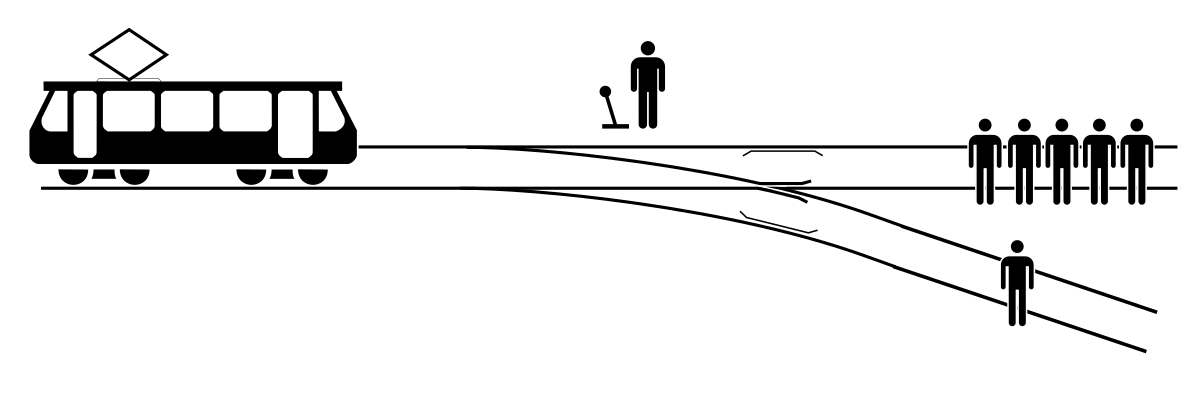
\includegraphics[scale=0.25]{Trolley_Problem.svg}
        \end{center}
        \label{fig:minAI}
    \end{figure}
\end{frame}

% Aleksandar

\section{Veštačka inteligencija u vojne svrhe}

\begin{frame}{Veštačka inteligencija u vojne svrhe}
    \begin{itemize}
    
        \item Veštačka inteligencija u vojne svrhe povlači etička pitanja
        \item \textbf{Međunarodno humanitarno pravo (IHL)} kao dodatna prepreka u razvoju etičkog softvera
        \item Veštačka inteligencija u vojne svrhe ima svoje negativne i pozitivne strane
        
    \end{itemize}
\end{frame}

\begin{frame}{Negativne strane}
    \begin{itemize}
        \item<1-> Problem odgovornosti: ko je odgovoran za dela veštačke inteligencije?
        \item<2-> Rešenje: odgovorna osoba koja odlučuje u krucijalnim trenucima
        \item<3-> Problem preprilagođenosti: nepredvidivo ponašanje algoritama usled loših trening podataka
        \item<4-> Rešenje: adekvatan odabir ulaznih podataka i algoritama za učenje, temeljno testiranje
    \end{itemize}
\end{frame}

\begin{frame}{Pozitivne strane}
    \begin{itemize}
        \item<1-> Lakše i brže osvajanje pomoću veštačke inteligencije \textbf{nije} pozitivna strana
        \item<2-> Etičko oružije u vidu \textbf{MaxAI} i \textbf{MinAI} jeste pozitivna strana
        \item<3-> MaxAI: ne izvodljiv u praksi, trudi se da što preciznije prati naređenja
        \item<4-> MinAI: naređenja koja krše zakone se jednostavno ne izvršavaju, moguće je zadavanje sekundarnog naređenja (failsafe)
    \end{itemize}    
\end{frame}

\begin{frame}{Primer etičkog oružija: MinAI}
    \begin{figure}[h!]
        \begin{center}
            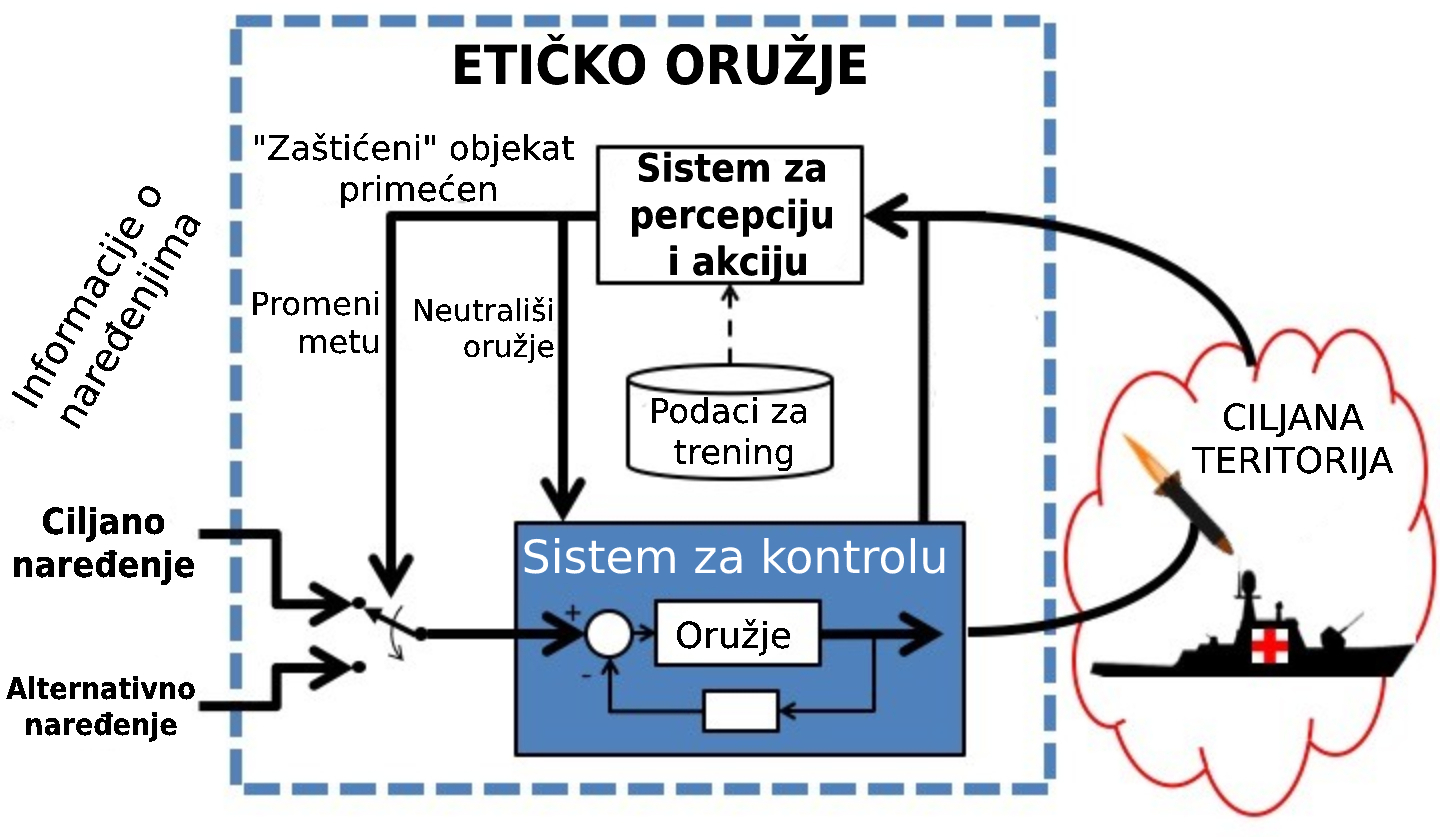
\includegraphics[scale=0.2]{minAI_slideovi.jpg}
        \end{center}
        \label{fig:minAI}
    \end{figure}
\end{frame}


\end{document}
